\lab{Applications}{Image Segmentation}{Image Segmentation}

\objective{Understand some basic applications of eigenvalues to graph theory}
\label{lab:ImgSeg_eigenvalues}

\section*{Graph Theory}
\begin{figure}

 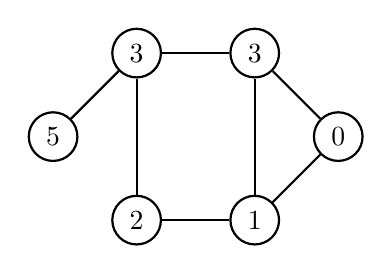
\begin{tikzpicture}[auto,node distance=1.5cm,
 thick,main node/.style={circle,draw}]

  \node[main node] (5) [] {5};
  \node[main node] (2) [below right of=5] {2};
  \node[main node] (3) [above right of=5] {3};
  \node[main node] (4) [right of=3] {3};
  \node[main node] (1) [right of=2] {1};
  \node[main node] (0) [below right of=4] {0};

  \foreach \s/\t in {5/3, 3/4, 4/0, 0/1, 1/2, 2/3, 1/4} {
   \path[draw] (\s) edge (\t);}
\end{tikzpicture}
\caption{A simple undirected graph}
\label{fig:example_graph}
\end{figure}

\begin{figure}
 \begin{tikzpicture}[->,>=stealth',shorten >=1pt,auto,node distance=1.5cm,
 thick,main node/.style={circle,draw}]

  \node[main node] (A) [] {A};
  \node[main node] (B) [below of=A] {B};
  \node[main node] (C) [right of=A] {C};
  \node[main node] (D) [below of=C] {D};
  \node[main node] (E) [right of=C] {E};
  \node[main node] (F) [right of=D] {F};

  \foreach \s/\t in {A/C, B/A, B/D, C/E, C/F, D/C} {
   \path[draw] (\s) edge (\t);}
\end{tikzpicture}
\caption{A simple directed graph}
\end{figure}



Graphs are often used to represent relationships between objects.
They are represented by a set of nodes (or vertices) and a set of edges, where each edge connects exactly two nodes.
We denote the number of vertices in a graph by $|V|$, and the number of edges by $|E|$.
A graph is \emph{directed} if connections are uni-directional, and \emph{undirected} if they are bi-directional.
One way to encode the information found in a graph is to use what is called an adjacency matrix.
\begin{definition} An adjacency matrix $A$ is a $|V| \times |V|$ matrix where the $(i,j)$-th entry $a_{ij}$ is
\begin{center}
	$a_{ij} = \begin{cases} 1 & \mbox{If an edge connects vertex i to vertex j} \\ 0 & \mbox{otherwise} \end{cases}$
\end{center}
%technically, the definition does not apply to all graphs (according to Wikipedia)
%however, this definition works if we are just considering simple graphs, i.e. at most one edge between any two vertices, no loops
\end{definition}

Every undirected edge can be represented as two directed edges.
Figure \ref{fig:example_graph} shows a simple undirected graph.
It can be represented by the following adjacency matrix.
\[
A = \begin{pmatrix}
0 & 1 & 0 & 0 & 1 & 0\\
1 & 0 & 1 & 0 & 1 & 0\\
0 & 1 & 0 & 1 & 0 & 0\\
0 & 0 & 1 & 0 & 1 & 1\\
1 & 1 & 0 & 1 & 0 & 0\\
0 & 0 & 0 & 1 & 0 & 0
\end{pmatrix}
\]
The adjacency matrix will always be symmetric for undirected graphs.
The diagonal represents self-edges, or edges that connect a node to itself.

Raising the adjacency matrix to a power yields some very interesting information.
We can discover the number of paths of length $n$ between two nodes by raising a graph's adjacency matrix to the $n$th power.
For example, by squaring $A$, we can find the number of paths of length two between every pair of nodes.
\begin{lstlisting}
>>> A = np.array([[0,1,0,0,1,0],[1,0,1,0,1,0],
                  [0,1,0,1,0,0],[0,0,1,0,1,1],
                  [1,1,0,1,0,0],[0,0,0,1,0,0]])

>>> np.linalg.matrix_power(A,2)
array([[2, 1, 1, 1, 1, 0],
       [1, 3, 0, 2, 1, 0],
       [1, 0, 2, 0, 2, 1],
       [1, 2, 0, 3, 0, 0],
       [1, 1, 2, 0, 3, 1],
       [0, 0, 1, 0, 1, 1]])
\end{lstlisting}
We can see that no paths of length two exist between node 0 and node 5 because $A^2_{0,5} = 0$.
By calculating $A^6$ we can find the number of paths of length six from node 3 to itself.
\begin{lstlisting}
>>> np.linalg.matrix_power(A, 6)
array([[45, 54, 38, 45, 54, 16],
       [54, 86, 29, 77, 51, 11],
       [38, 29, 55, 15, 70, 27],
       [45, 77, 15, 75, 31,  4],
       [54, 51, 70, 31, 93, 34],
       [16, 11, 27,  4, 34, 14]])
\end{lstlisting}
We see that there are 75 unique paths of length six from node 3 to itself.
Imagine trying to count all of those paths by hand!
It would be very easy to count incorrectly.
This method makes it very simple to count paths without mistakes.

Adjacency matrices can also be composed of \li{True} and \li{False} values.
In this case, the $n$th power of such a matrix (using boolean arithmetic)
is again a matrix of
boolean values which simply indicate whether there exists a path of length $n$ between the given pair of nodes, rather than indicating the number of such
paths.

\begin{problem}
Let the following matrix represent a directed graph
\[
\begin{pmatrix}
0 & 0 & 1 & 0 & 1 & 0 & 1 \\
1 & 0 & 0 & 0 & 0 & 1 & 0 \\
0 & 0 & 0 & 0 & 0 & 1 & 0 \\
1 & 0 & 0 & 0 & 1 & 0 & 0 \\
0 & 0 & 0 & 1 & 0 & 0 & 0 \\
0 & 0 & 1 & 0 & 0 & 0 & 1 \\
0 & 1 & 0 & 0 & 0 & 0 & 0
\end{pmatrix}
\]
Between which pair of nodes does there exist the greatest number of paths
of length five?
From which node to which node is there no path of length seven?
\end{problem}

An important question in working with graphs is the degree of its nodes.
The degree of a node is the number of edges that connect to the node.
For a directed graph, each node has an \emph{out-degree} (the number of edges directed away from a node) and an \emph{in-degree} (the number edges directed toward a node).
The \emph{degree matrix} of a graph is a diagonal matrix that has the degree of each node as the diagonal entries (thus, for a directed graph there is an in-degree matrix and an out-degree matrix).

Another useful way of representing an undirected graph is a \emph{Laplacian matrix}.
This special matrix can reveal a lot of information about a graph, which we will see later in this lab.
\begin{definition}
For a simple graph (an undirected graph without self-edges), the Laplacian of a graph $G$ is
\[ L_G = D_G - A_G \]
where $D_G$ is the degree matrix of $G$ and $A_G$ is the adjacency matrix of $G$.
\end{definition}


\begin{problem}
Write a function that accepts the adjacency matrix of a graph as an argument. Use the adjacency matrix to check that the graph is undirected and has no self-edges. Then using the definition above, calcluate the Laplacian matrix.

Test your function by finding the Laplacian matrix of the graph in Figure \ref{fig:example_graph}. Your function should return the following Laplacian matrix:
\[
\begin{pmatrix}
2 &-1 & 0 & 0 &-1 & 0 \\
-1 & 3 &-1 & 0 &-1 & 0 \\
0 &-1 & 2 &-1 & 0 & 0 \\
0 & 0 &-1 & 3 &-1 &-1 \\
-1 &-1 & 0 &-1 & 3 & 0 \\
0 & 0 & 0 &-1 & 0 & 1 \\
\end{pmatrix}
\]
\label{prob:laplacian}
\end{problem}


We may also define \emph{weighted graphs} so that each edge has a weight or cost attached to it.
In this case, the entries of the adjacency matrix are the costs, rather than just ones or zeros.
An example of a weighted graph could be a collection of cities as vertices, roads connecting them as edges, and the distances of the connecting roads as the costs attached to each edge.

In this lab we will learn about the information we can discover about a graph from examining the spectrum of its adjacency matrix and its Laplacian.
While the formulation of the Laplacian matrix seems to be very simple, its structure allows us to learn surprising things by examining its eigenvalues.

For a weighted graph the definition of the Laplacian is as follows.

\begin{definition}  The \emph{degree} of a vertex of a weighted graph is the sum of the weights of the edges connected to that vertex.
In undirected graphs, which is what we will be dealing with, this is the sum of all the weights moving into that vertex.
This definition varies slightly for directed graphs.
Let $D$ be a diagonal matrix with
\[
D_{ii} = \mbox{ Degree of vertex $i$}
\]
and let $A$ be the adjacency matrix of the graph.
The graph \emph{Laplacian} $Q$ is given by
\[
Q = D-A
\]
\end{definition}

The Laplacian matrix of a graph will typically be very sparse.

A \emph{connected graph} is a graph where every vertex is connected to every other vertex by at least one path.
An important question one might ask about a graph is whether or not it is connected.
What is the best way to do this?
A naive approach would be to exhaustively map every possible path from each vertex.
While this would be feasible for very small graphs, most interesting graphs (for example, the internet) will have thousands of vertices, and such an approach becomes essentially impossible to execute.

It turns out there is a better way.
If the second smallest eigenvalue of the Laplacian matrix associated with a graph is positive, then this graph is connected.
The mathematics behind this is quite involved, so we omit a proof for now.
In many applications the Laplacian matrix will be very sparse, and thus with optimizations made for sparsity, we can discover the connectivity of a graph relatively cheaply.

\begin{problem}Write a function \li{laplacian} that accepts an adjacency matrix as an argument and returns the Laplacian matrix and its second smallest eigenvalue.
Use the \li{scipy.linalg} package to compute the eigenvalue.

Use \li{numpy.random.rand(n,n)} to generate two random matrices of sizes n=10 and n=100.
Then use masking to change the sparsity of each of the matrices, i.e. \li{numpy.random.rand(n,n) > c} for \li{c = 0.25,0.95}. This will create four different matrices of boolean values. Remember that when doing calculations with boolean values that \li{True} is considered to be a 1 and \li{False} is considered to be a 0. Is the n=10 adjacency matrix connected when we let c=.25? What about when we let c=.95? Is the n=100 adjacency matrix connected when c=.95?
\end{problem}


\section*{Image Segmentation}

\begin{figure}
    \centering
    \begin{subfigure}{0.31\textwidth}
        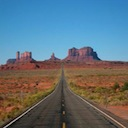
\includegraphics[width=\textwidth]{RegMon.png}
    \end{subfigure}
   \hspace*{\fill}
    \begin{subfigure}{0.31\textwidth}
        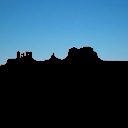
\includegraphics[width=\textwidth]{NegMon.png}
    \end{subfigure}
    \hspace*{\fill}
    \begin{subfigure}{0.31\textwidth}
        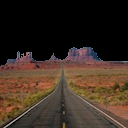
\includegraphics[width=\textwidth]{PosMon.png}
    \end{subfigure}
    
\caption{An image and its segments.}
\label{fig:monument}
\end{figure}

An important problem in image processing is that of image segmentation.
When humans observe an image, they can easily pick out portions of that image that ``belong together''.
For example, if we saw a picture of a person against a black background, the pixels making up the background would make up one segment of the image, and the person would make up the other part.
While this seems simple for a human, how can we program a computer to do so? (See Figure \ref{fig:monument} for an example of a segmented image).

One way to do this was presented in a paper by Jianbo Shi and Jitendra Malik in 2000. To use the algorithm they presented, we first need to find the adjacency matrix of an image.
An image is a collection of coordinates and light intensities.
We call each coordinate and associated brightness a pixel.
We let every pixel in an image be a vertex in a graph that is connected to its neighbors within a certain radius.
For an $N \times N$ image, we define an adjacency matrix as follows:

\begin{equation}
\label{eq:adjacency}
w_{ij} = e^{-\frac{|I(i) - I(j)|}{\sigma_I^2}} \cdot \begin{cases} e^{-\frac{d(i,j)}{\sigma_d^2}} & \mbox{ for $d(i,j) < r$} \\ 0 & \mbox{ otherwise} \end{cases}
\end{equation}
for $i = 1 \hdots N^2$ and $j = 1 \hdots N^2$ (where both $i$ and $j$ travel through each pixel in the image), and where
\begin{itemize}
	\item$d(i,j)$ is the Euclidean distance between pixel $i$ and pixel $j$
	\item $|I(i) - I(j)|$ is the difference in brightness of pixels $i$ and $j$
	\item $\sigma_I$ and $\sigma_d$ are constants
	\item $r$ is the radius
\end{itemize}
Thus, given a $N\times N$ image, we will produce an adjacency matrix of size $N^2\times N^2$.
Even for smaller images, this will become very large, but we have sparsity on our side, especially if $r$ is small. Even so, only do this for images smaller than 50 by 50.

In definition \eqref{eq:adjacency}, we can think of $w_{ij}$ as the weight representing the similarity between pixels. So if a weight between two pixels is low, we can think of those pixels as being less similar and therefore more likely to represent where the image is segmented. We therefore want to segment our image along the edges with low weights. The total weight of the edges we remove is called the `cut' and so part of the mathematics behind image segmentation is minimizing the `cut', or in other words finding the segments that are least similar to each other.



In the following problem we will write a function that finds the adjacency matrix of an image, based on the definition from \eqref{eq:adjacency}. To do this, we first flatten the image we are working on. 

\begin{lstlisting}
nodes = img.flatten()
\end{lstlisting}

This allows us to index all of the pixels (or nodes) using a one-dimensional array. By doing this, we are better able to calculate the weights in-between pixels. It is important to note here that this is only one way of indexing the pixels in our image. We can still index the pixels in our image or matrix by using standard tuple notation. So for example, given a $2 \times 2$ matrix we can access the bottom-right element (if we are starting at row 0 and column 0) by the tuple (1,1). If we choose to flatten our matrix we can index the same element by the number 3 (if we once again start at 0).

Since each pixel is only connected to the pixels within radius $r$, relatively few entries of our adjacency matrix will be non-zero. For this reason, we will work with sparse matrices from the \li{scipiy.sparse} package. We first initialize our adjacency matrix as a sparse matrix.

\begin{lstlisting}
W = spar.lil_matrix((nodes.size, nodes.size), dtype=float)
\end{lstlisting}
We use \li{lil_matrix} because it gives us an efficent way to build our matrix piece by piece. To learn more about sparse matrices in scipy read the documentation at \url{http://docs.scipy.org/doc/scipy/reference/sparse.html}.

At this point we can initialize the main diagonal of the degree matrix. We only care about the main diagonal because the degree matrix is a diagonal matrix.
\begin{lstlisting}
D = np.zeros((1, nodes.size))
\end{lstlisting}
Now we go through each pixel of our image matrix to calculate the weights.

\begin{lstlisting}
# 'height' is the original height of the image
# 'width' is the original width of the image
for row in xrange(height):
    for col in xrange(width):
        # Calculate the index of the pixel at (row, col) relative to the
        # flattened array 'nodes'. 
        rowcol = row * width + col
\end{lstlisting}
Say we start with pixel \li{A}. Notice that we do not need to find the weights between every pixel and pixel \li{A}, since most of the weights will be 0. We only need to find the weights between pixel \li{A} and those pixels that are within radius $r$ of pixel \li{A}. 

A helper function has been provided that finds the pixels and corresponding distances within radius $r$ of a single pixel. Note that the pixel being passed into the function is indexed as a tuple, or more precisely as a given row and column index. The function returns however, an array of indices in the flat array form (single numbers) of pixels within radius $r$ of the pixel passed into the function.
\lstinputlisting[style=fromfile]{getNeighbors.py}
Below we use the helper function to get the indices and distances.

\begin{lstlisting}
# find the indices and distances of the pixels that are within 
# distance r of the current pixel by calling getNeighbors
indices, distances = getNeighbors(row, col, radius, height, width)
\end{lstlisting}
We can then calcluate the weights between pixels by using definition \eqref{eq:adjacency}. The helper function already calculates the distances, so now we just need to find the difference in brightness of pixels by subtracting the corresponding pixels.
Once we find the weights we can then add them into our adjacency matrix. 
\begin{lstlisting}
# 'weights' is the weights between the pixel we are on and the pixels within
# radius r
W[rowcol, indices] = weights
\end{lstlisting}
We can also calculate part of the main diagonal of the degree matrix.
\begin{lstlisting}
D[0,rowcol] = weights.sum()
\end{lstlisting}
We now loop to the next pixel and repeat the process.

After we have found our adjacency matrix (\li{W} in the code we have provided above) we convert it to a \li{csc} format, and return both \li{W} and \li{D}. 
\begin{lstlisting}
W = W.tocsc()
return W, D
\end{lstlisting}
The sparse matrix format \li{csc} is better for computations which we will want to use later.




\begin{problem}
Write a function \li{adjacency} that takes an $N \times N$ image array, radius $r$, and values for
$\sigma_I^2$ and $\sigma_d^2$, and returns the adjacency matrix defined in \eqref{eq:adjacency}. Test your function on the image \li{dream.png}. This image is read in as a color photo so first convert it to grayscale to reduce it to two dimensions.
\begin{lstlisting}
# read in the image
img_color = plt.imread('dream.png')
# convert to grayscale
img = (img_color[:,:,0]+img_color[:,:,1]+img_color[:,:,2])/3.0
\end{lstlisting}
Let $r=5.0$, $\sigma_I^2=0.02$ and $\sigma_d^2=3.0$.


%Notice that for each pixel you can save time by only checking the pixels $r$ rows and columns away.
%For that you'll have to handle the pixels on the edges and corners of the image carefully.
%I gave them new helper code, which abstracts away the edge cases.
\label{prob:adjacency_dream}
\end{problem}

As was mentioned before, we are trying to minimize the `cut', or the total weight of the edges we remove to create segments. This problem comes down to finding the second smallest eigenvalue of $D^{-1/2}QD^{-1/2}$, where $D$ is the degree matrix and $Q$ is the Laplacian matrix of the adjacency matrix defined in \eqref{eq:adjacency}. The mathematics behind this is quite involved, so the reader is encouraged to read the paper that Shi and Malik wrote at \url{http://www.cs.berkeley.edu/~malik/papers/SM-ncut.pdf} for a better understanding.
	
To calculate $D^{-1/2}QD^{-1/2}$, we once again use sparse matrices. We use the \li{adjacency} function from Problem \ref{prob:adjacency_dream} to find the adjacency matrix \li{W} and the main diagonal of the degree matrix \li{D}. We can convert \li{D} into a diagonal sparse matrix using \li{spar.spdiags}.

\begin{lstlisting}
Ds = spar.spdiags(D, 0, D.shape[1], D.shape[1], format = 'csc')
\end{lstlisting}

In like manner we can find the diagonal sparse matrix $D^{-1/2}$. We can also calculate the Laplacian matrix $Q$ since \li{Ds} and \li{W} are both sparse matrices and in `csc' format. To matrix multiply two sparse matrices together, use the \li{dot} function. For example, if \li{M} and \li{N} are two sparse matrices, use \li{M.dot(N)}.

The eigenvector associated with the second smallest eigenvalue will be a $N^2 \times 1$ vector and will have positive and negative entries. If we reshape this vector to be the same size as our original image we can create a mask that will create two segments - one segment corresponding to the positive values of the eigenvector and the other segment corresponding to the negative values of the eigenvector. 

\begin{lstlisting}
# create a mask array that is True wherever the eigenvector is positive.
# reshape it to be the size of img.
mask = (eigvec>0).reshape(img.shape)
\end{lstlisting}
To find the segments, we only need to take the product of our mask with the original image.

\begin{lstlisting}
# create the positive segment by masking out the pixels in img 
# belonging to the negative segment.
pos = img*mask
\end{lstlisting}
By recursively executing this function, we can find segments within segments.


\begin{problem}  Write a function \li{segment} that solves the segmentation problem for small images.
Accept an image array as an argument and return the two segments.
Use $r = 5.0, \sigma_I^2 = 0.02,$ and $\sigma_d^2 = 3.0$.
Remember that the Laplacian matrix will be very large, but also very sparse.
Because of the way we defined $\sigma_I^2$ the image matrix intensity values need to be between $0.0$ and $1.0$. If this is not standard for the images you are using, change $\sigma_I^2$.

Test your function on the image \li{dream.png}. Your segments should look like the segments in Figure \ref{fig:dream_solution} with the original image on the left.
\end{problem}

\begin{figure}
\centering
    \centering
    \begin{subfigure}{0.31\textwidth}
        
\includegraphics[width=\textwidth]{RegDream.png}
    \end{subfigure}
    \hspace*{\fill}
    \begin{subfigure}{0.31\textwidth}
        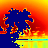
\includegraphics[width=\textwidth]{NegDream.png}
    \end{subfigure}
    \hspace*{\fill}
    \begin{subfigure}{0.31\textwidth}
        
\includegraphics[width=\textwidth]{PosDream.png}
    \end{subfigure}
\caption{Segments of \li{dream.png}}
\label{fig:dream_solution}
\end{figure}